%%%%%%%%%%%%%%%%%%%%%%%%%%%%%%%%%%%%%%%%%%%%%%%%%%%%%%%%%%%%%%%%%%%%%%%%%%%%%%%%%%%%%
%
%
%
%
%%%%%%%%%%%%%%%%%%%%%%%%%%%%%%%%%%%%%%%%%%%%%%%%%%%%%%%%%%%%%%%%%%%%%%%%%%%%%%%%%%%%%
\documentclass[12pt]{article}
%
\usepackage[a4paper]{geometry}
\usepackage[slovene,english,german]{babel}
\usepackage[T1]{fontenc}
\usepackage[cp1250]{inputenc}
\usepackage{graphicx}
\usepackage{bchart}
\usepackage{fancyhdr}
\usepackage{gensymb}
\usepackage{wrapfig}
\usepackage[export]{adjustbox}
\usepackage{amsmath}
\addtolength{\textheight}{1cm}
%
%

\author{Jaka �op}
\title{Terenska vaja - naravnogeografska \\ Kemi�ne lastnosti vode}
%
\begin{document}
\selectlanguage{slovene}
\pagenumbering{gobble}
  \maketitle

Na vajo smo se kot pri prej�nji delno pripravili �e v �oli, ker so priprave potekale zelo podobno kot pri pri vaji jih tu ne bom podrobno opisoval.

Vaja je ob lepem vremenu potekala zelo gladko. Po zajetju vode iz zatoka in morja sem ju najprej primerjal z destilirano. Vse vode so se po barvi malenkostno razlikovale kar me je mo�no presenetilo saj sem pri�akoval, da bo voda v sju�i precej bolj onesna�ena kot voda iz morja. Vonj obeh vod je bil slab, vonj vode iz morja pa celo zelo slab. Voda iz morja je imela zelo slab vonj po ribah, medtem ko je imela voda iz stju�e malenkost mo�nej�i vonj po zemlji. Po vonjanju obeh vod sem vodama izmeril pH in dobil slede�e rezultate. Voda iz zatoka je imela pH 6, voda iz morja pa 7. Za konec vaje sem vodo �e prefiltriral. To je bil vsaj za moj okus najdolgo�asnej�i del vaje, saj se je voda filtrirala neizmerno po�asi. Za povrh vsega pa je na filtrirnem papirju komaj ostalo kaj vidnega, kot so: manj�e smetke, nekaj ve�jih, majhna �ivalca, v vodi iz zatoka ter le nekaj manj�ih smetk v vodi iz morja.

Iz pridobljenih rezultaov lahko sklepam, da tako morje kot zatok (pri�akoval sem, da bo zatok precej onesna�en predvsem iz prej�njih izku�enj) nista zelo onesna�ena, kar je seveda prijetno presene�enje.

\begin{figure}[!htbp]
  \centering
  % Requires \usepackage{graphicx}
  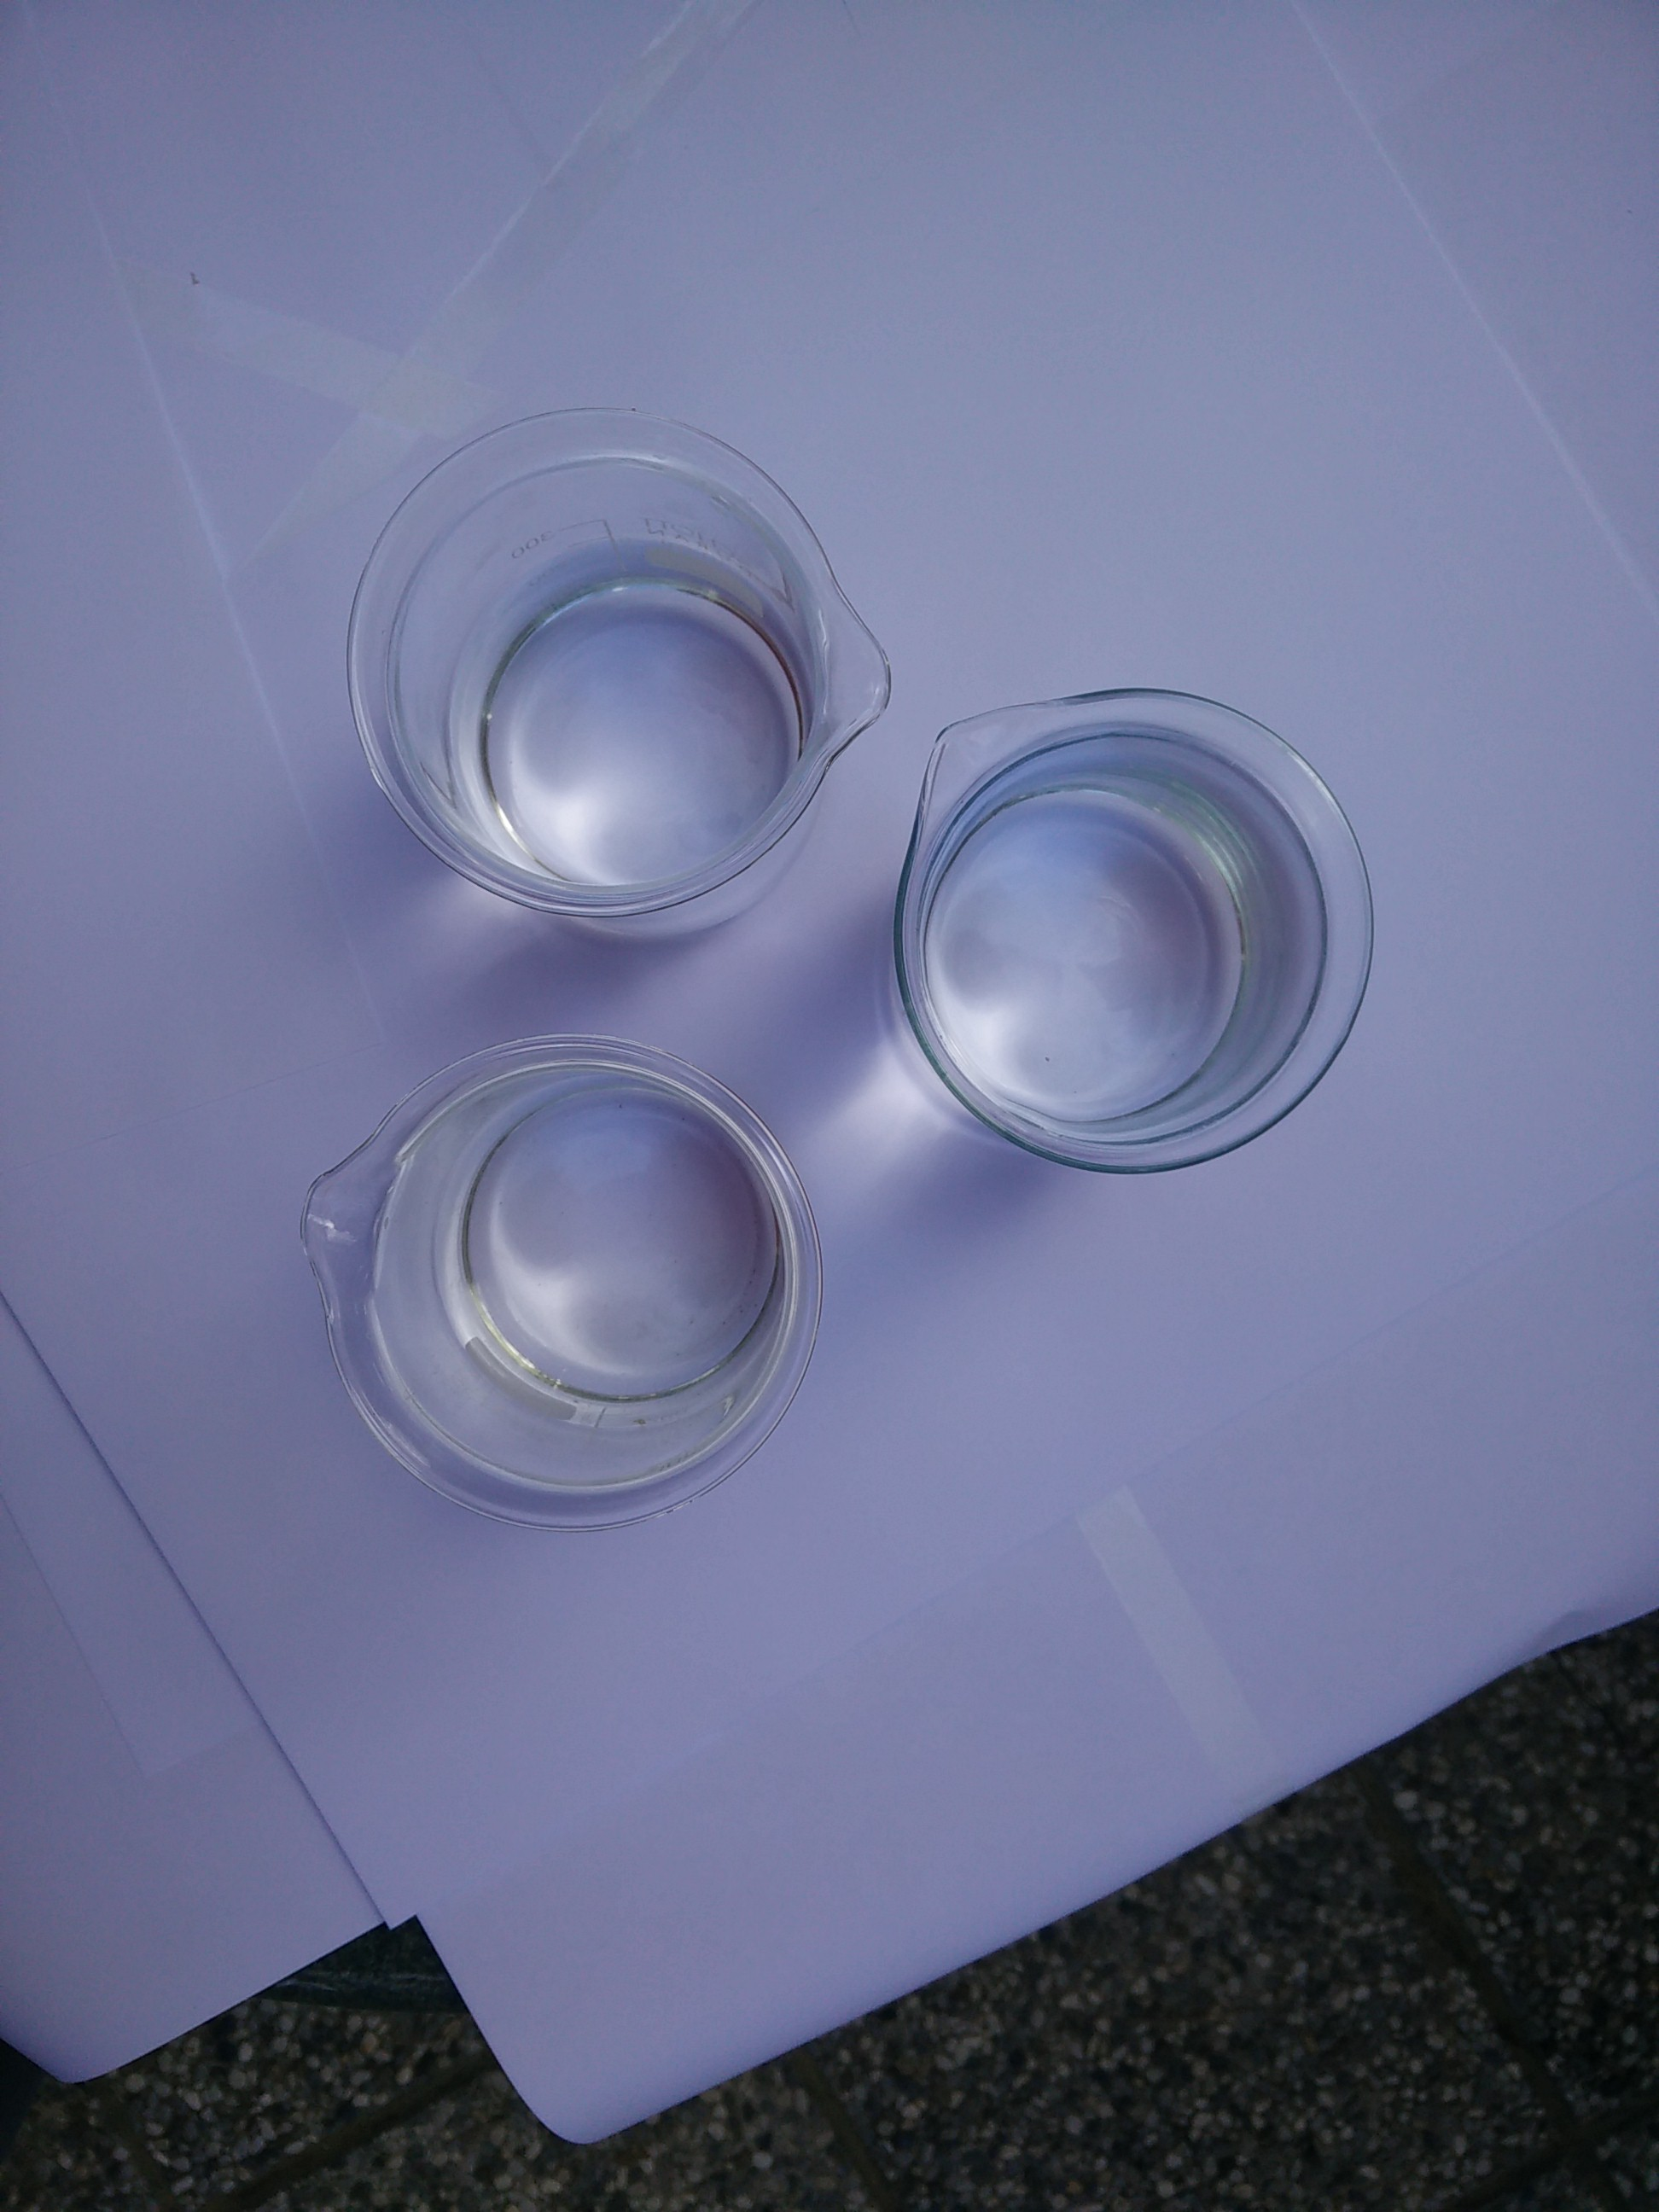
\includegraphics[width=.9\textwidth]{./Slike/vode.jpg}\\
  \caption{Primerjava vseh treh vod (na vrhu destilirana voda, desno voda iz zatoka ter spodaj voda iz morja), kot lahko vidimo so razlike minimalne}\label{vode}
\end{figure}

\end{document} 